Outlined below are some coding fragments categorised under: Design Patterns, Asynchronous Tasks, Presenters, Views and Interesting Coding Fragments.

\subsection*{Design Patterns}
\subsubsection*{DAOFactory class}
\begin{lstlisting}[style=Java]
public class DAOFactory {

    public DAO getDAO(Context context){
        return SqlLiteDAO.getInstance(context);
    }
}
\end{lstlisting}

\subsubsection*{DAO interface}
\begin{lstlisting}[style=Java]
public interface DAO {
    void addFoodLog(FoodLog foodLog);
    List<FoodLog> getLogsByDay(Date date);
    List<FoodLog> getLogsByWeek(Date date);
    List<FoodLog> getLogsByMonth(Date date);
    void deleteFoodLogs(List<FoodLog> foodLogs);
    void deleteDb();
}
\end{lstlisting}

\subsubsection*{HostFactory class}
\begin{lstlisting}[style=Java]
public class HostFactory {

    public Host createHost() {
        Host host = new Host.HostBuilder("52.214.205.157")
                    .withDns("ec2-52-214-205-157.eu-west-1.compute.amazonaws.com")
                    .withPort(5000)
                    .withRoute("/classifyImage/")
                    .build();
        return host;
    }
}
\end{lstlisting}

\subsubsection*{HostBuilder}
\begin{lstlisting}[style=Java]
public static class HostBuilder {
    private final String ipv4;
    private String dns;
    private int port;
    private String route;

    public HostBuilder(String ipv4) {
        this.ipv4 = ipv4;
    }

    public HostBuilder withDns(String dns) {
        this.dns = dns;
        return this;
    }

    public HostBuilder withPort(int port) {
        this.port = port;
        return this;
    }

    public HostBuilder withRoute(String route) {
        this.route = route;
        return this;
    }

    public Host build() {
        return new Host(this);
    }

}
\end{lstlisting}

\subsubsection*{Singleton DAO Object}
\begin{lstlisting}[style=Java]
public static DAO getInstance(Context context) {
    if(instance == null) {
        instance = new SqlLiteDAO(context);
    }
    return instance;
}
\end{lstlisting}

\subsection*{Asynchronous Tasks}
\subsubsection*{Send image to server - AsyncTask}
\begin{lstlisting}[style=Java]
@Override
protected String doInBackground(Void... params) {
    String result = "";
    OkHttpClient client = new OkHttpClient();
    String imageToSend = image;
    RequestBody requestBody = new MultipartBody.Builder()
            .setType(MultipartBody.FORM)
            .addFormDataPart("image", imageToSend)
            .build();

    Request request = new Request.Builder().url(host.getUrl())
            .post(requestBody).build();

    Response response = null;
    try {
        response = client.newCall(request).execute();
        result = response.body().string();
        response.body().close();
    } catch (IOException e) {
        e.printStackTrace();
    }

    return result;
}
\end{lstlisting}

\subsubsection*{Get Calories from API - AsyncTask}
\begin{lstlisting}[style=Java]
@Override
protected String doInBackground(Void... params) {
    String result = "";
    OkHttpClient client = new OkHttpClient();

    Request request = new Request.Builder().url(url)
            .build();

    Response response = null;
    try {
        response = client.newCall(request).execute();
        result = response.body().string();
        response.body().close();
    } catch (IOException e) {
        e.printStackTrace();
    }
    try {
        JSONObject jsonObject = new JSONObject(result);;
        JSONArray jsonArray = jsonObject.getJSONArray("hits");
        JSONObject hits = jsonArray.getJSONObject(0);
        JSONObject fields = hits.getJSONObject("fields");
        String calories = fields.getString("nf_calories");
        result = calories;
    } catch (JSONException e) {
        e.printStackTrace();
    }
    return result;
}
\end{lstlisting}

\subsection*{Presenters}
\subsubsection*{Presenter for Main Activity}
\begin{lstlisting}[style=Java]
public class MainPresenter {

    private Intent intent;
    private Context context;

    public MainPresenter(Context context) {
        this.context=context;
    }

    public void takePhoto() {
        intent = new Intent(context, CaptureImageActivity.class);
        context.startActivity(intent);
    }

    public void userLogs() {
        intent = new Intent(context, FoodLogsActivity.class);
        context.startActivity(intent);
    }

}
\end{lstlisting}

\subsection*{Views}
\subsubsection*{Main Activity}
\begin{lstlisting}[style=Java]
public class MainActivity extends AppCompatActivity {

    private MainPresenter mainPresenter;

    @Override
    protected void onCreate(Bundle savedInstanceState) {
        super.onCreate(savedInstanceState);
        setContentView(R.layout.activity_main);

        mainPresenter = new MainPresenter(this);
    }

    public void onClickTakePhoto(View view) {
        mainPresenter.takePhoto();
    }

    public void onClickUserLogs(View view) {
        mainPresenter.userLogs();
    }
}
\end{lstlisting}

\subsection*{Interesting Coding Fragments}

\subsubsection*{Encode Bitmap to base64 String}
\begin{lstlisting}[style=Java]
public String toBase64() {
    BitmapFactory.Options options = new BitmapFactory.Options();
    options.inSampleSize = 8;

    Bitmap imageBitmap = BitmapFactory.decodeFile(image.getAbsolutePath(), options);

    //resize image for faster upload to server
    Bitmap.createScaledBitmap(imageBitmap, 300, 400, false);
    
    ByteArrayOutputStream byteArrayOutputStream = new ByteArrayOutputStream();
    imageBitmap.compress(Bitmap.CompressFormat.PNG, 100, byteArrayOutputStream);
    byte[] byteArray = byteArrayOutputStream.toByteArray();

    return Base64.encodeToString(byteArray, Base64.DEFAULT);
}
\end{lstlisting}

\subsection*{User Interface}
User interface implementation as in Figures \ref{fig:ui1}, \ref{fig:ui2}, \ref{fig:ui3}, \ref{fig:ui4}, \ref{fig:ui5}, \ref{fig:ui6}, \ref{fig:ui7} and \ref{fig:ui8}.

\begin{figure}[h] 
  \label{uiDesign1} 
  \begin{minipage}[b]{0.5\linewidth}
    \centering
    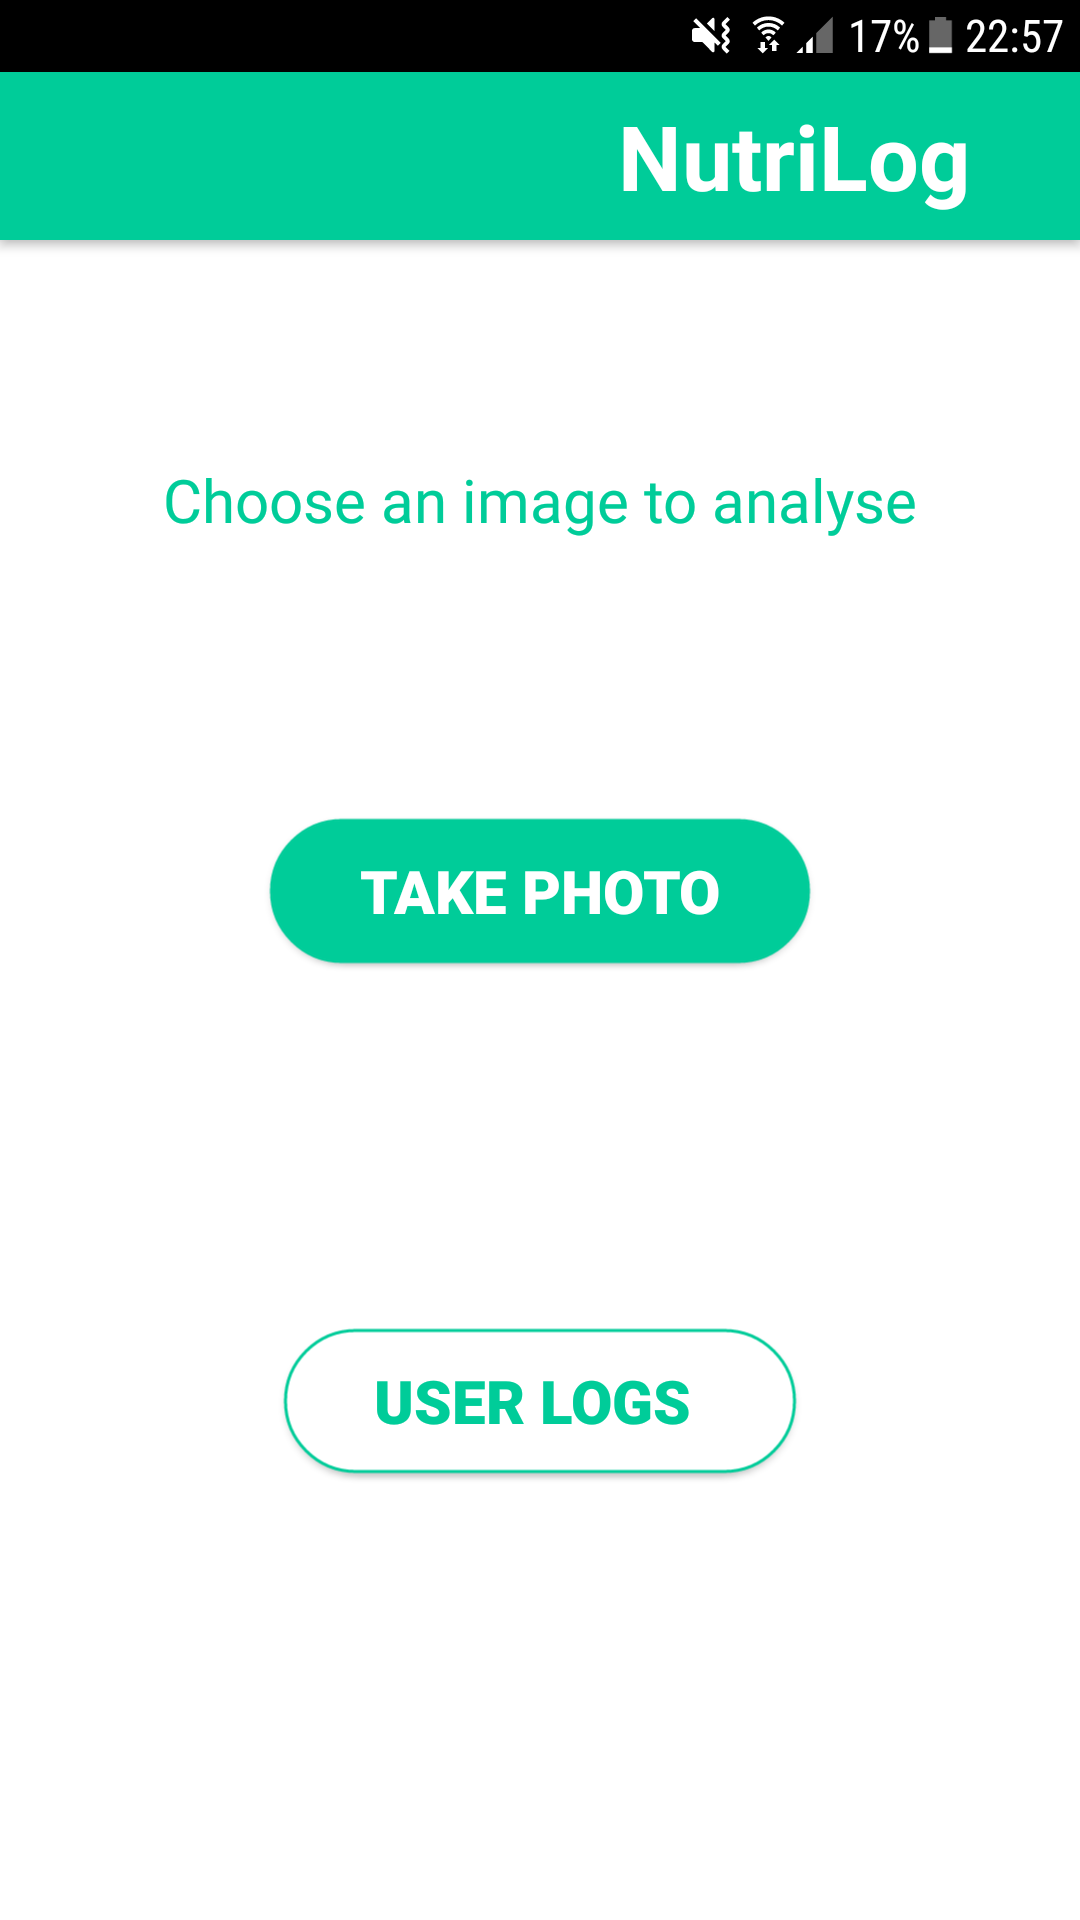
\includegraphics[width=.75\linewidth]{ui1} 
    \caption{Landing Activity} 
  \label{fig:ui1}
    \vspace{4ex}
  \end{minipage}%%
  \begin{minipage}[b]{0.5\linewidth}
    \centering
    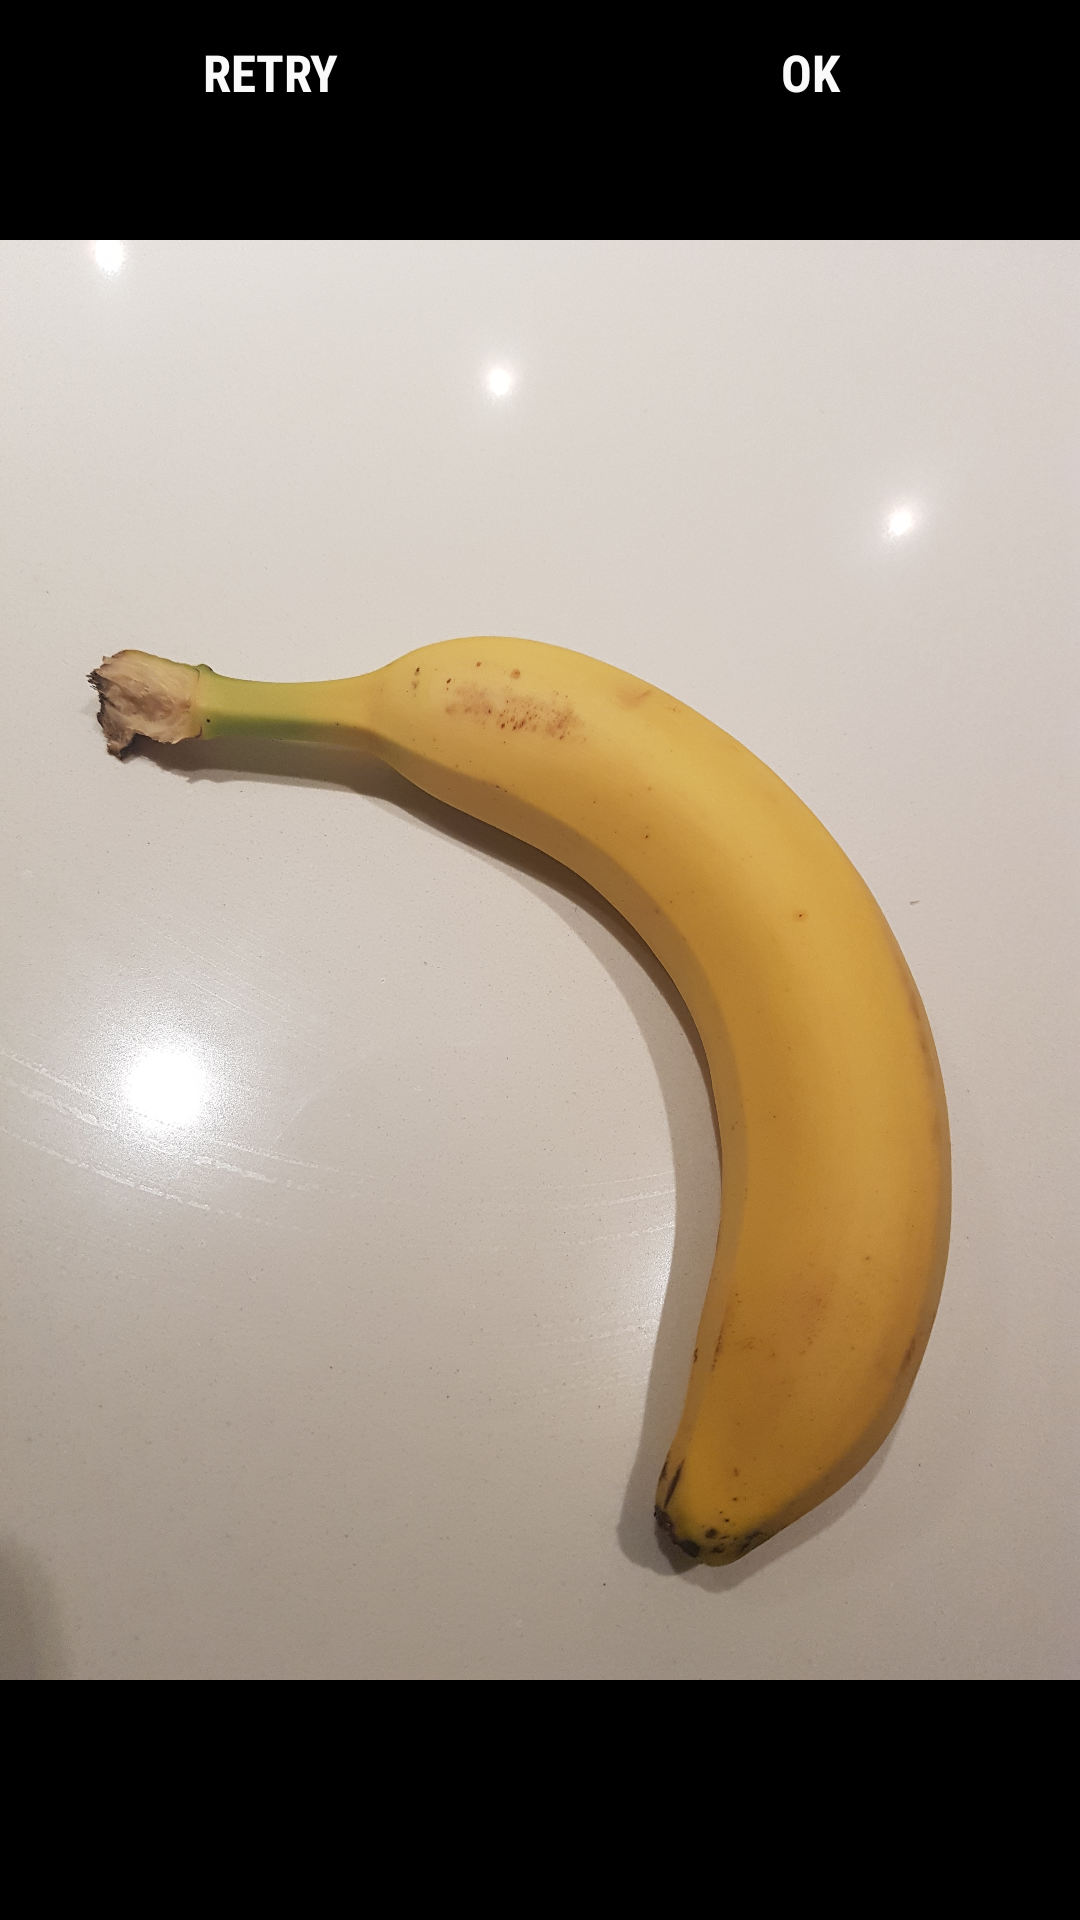
\includegraphics[width=.75\linewidth]{ui2} 
    \caption{Image Capture Activity} 
  \label{fig:ui2}
    \vspace{4ex}
  \end{minipage} 
  \begin{minipage}[b]{0.5\linewidth}
    \centering
    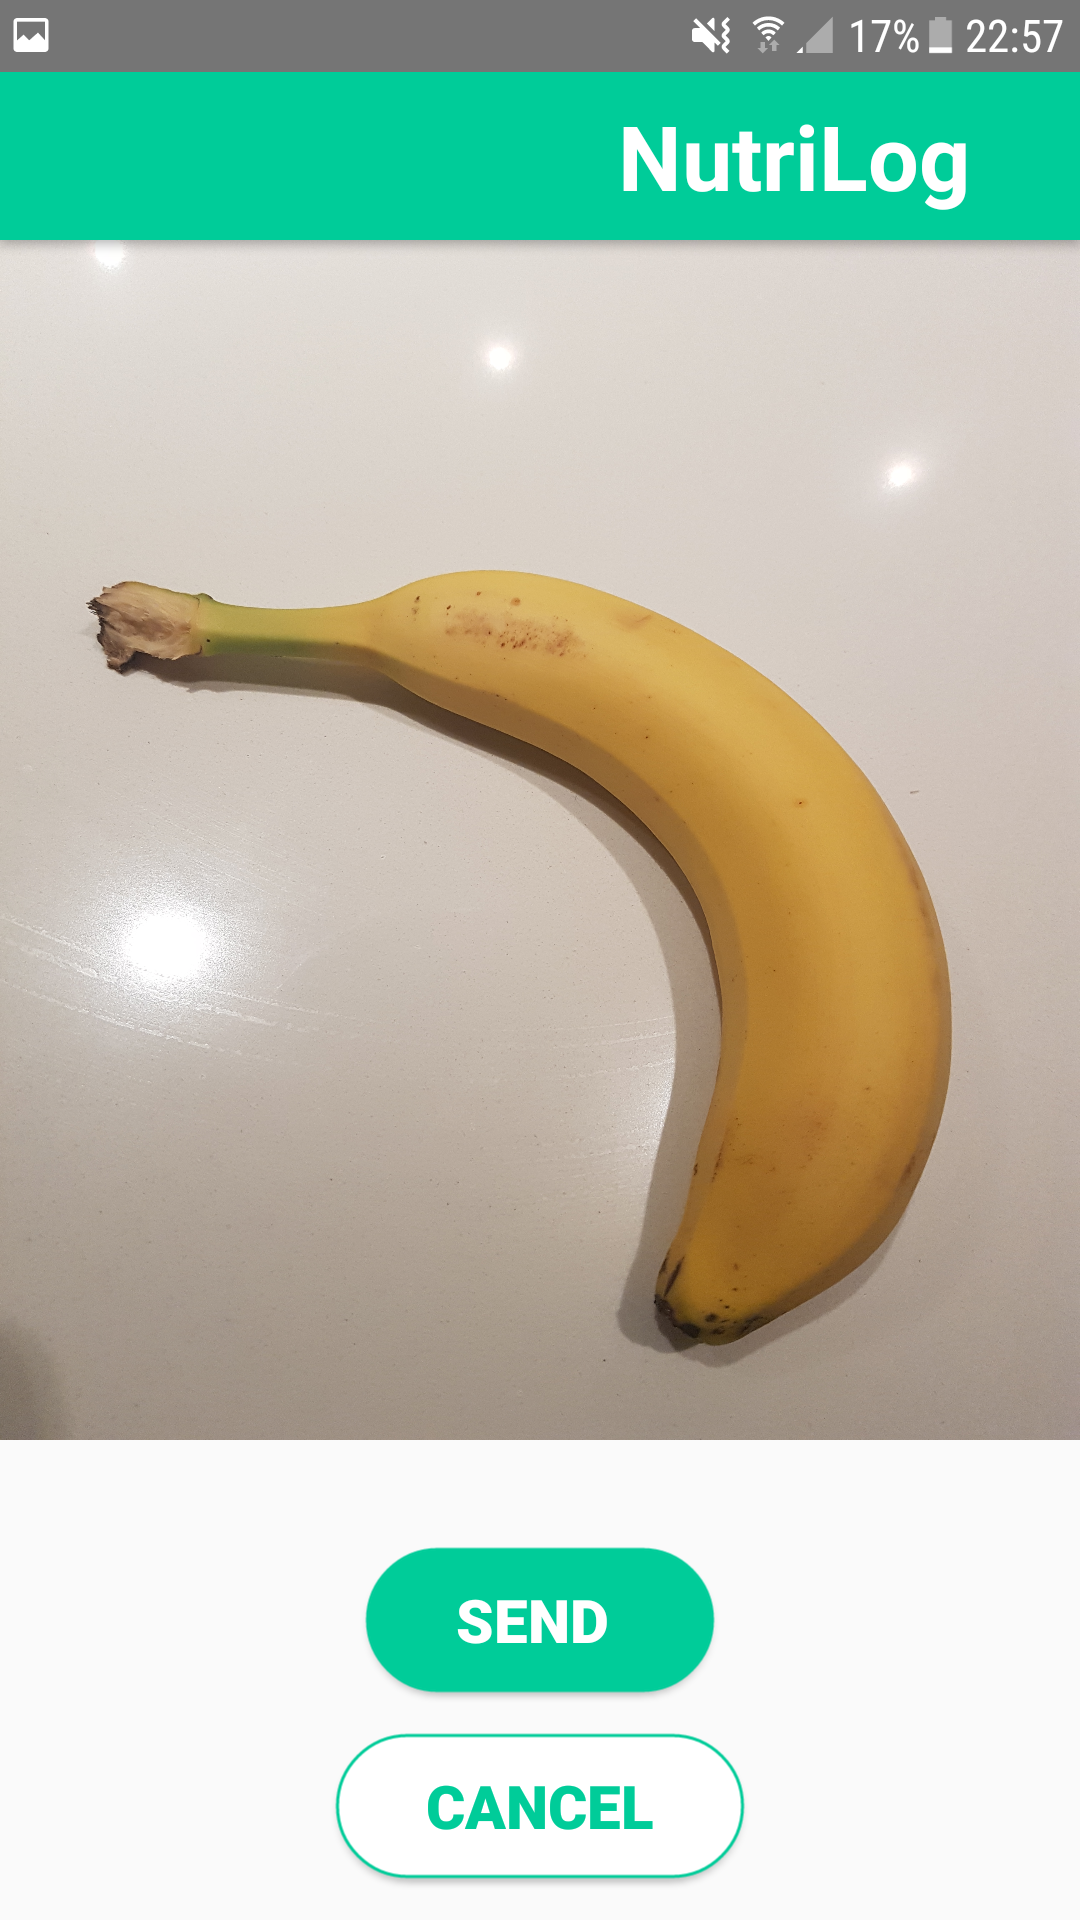
\includegraphics[width=.75\linewidth]{ui3} 
    \caption{Image Send Activity} 
    \label{fig:ui3}
    \vspace{4ex}
  \end{minipage}%% 
  \begin{minipage}[b]{0.5\linewidth}
    \centering
    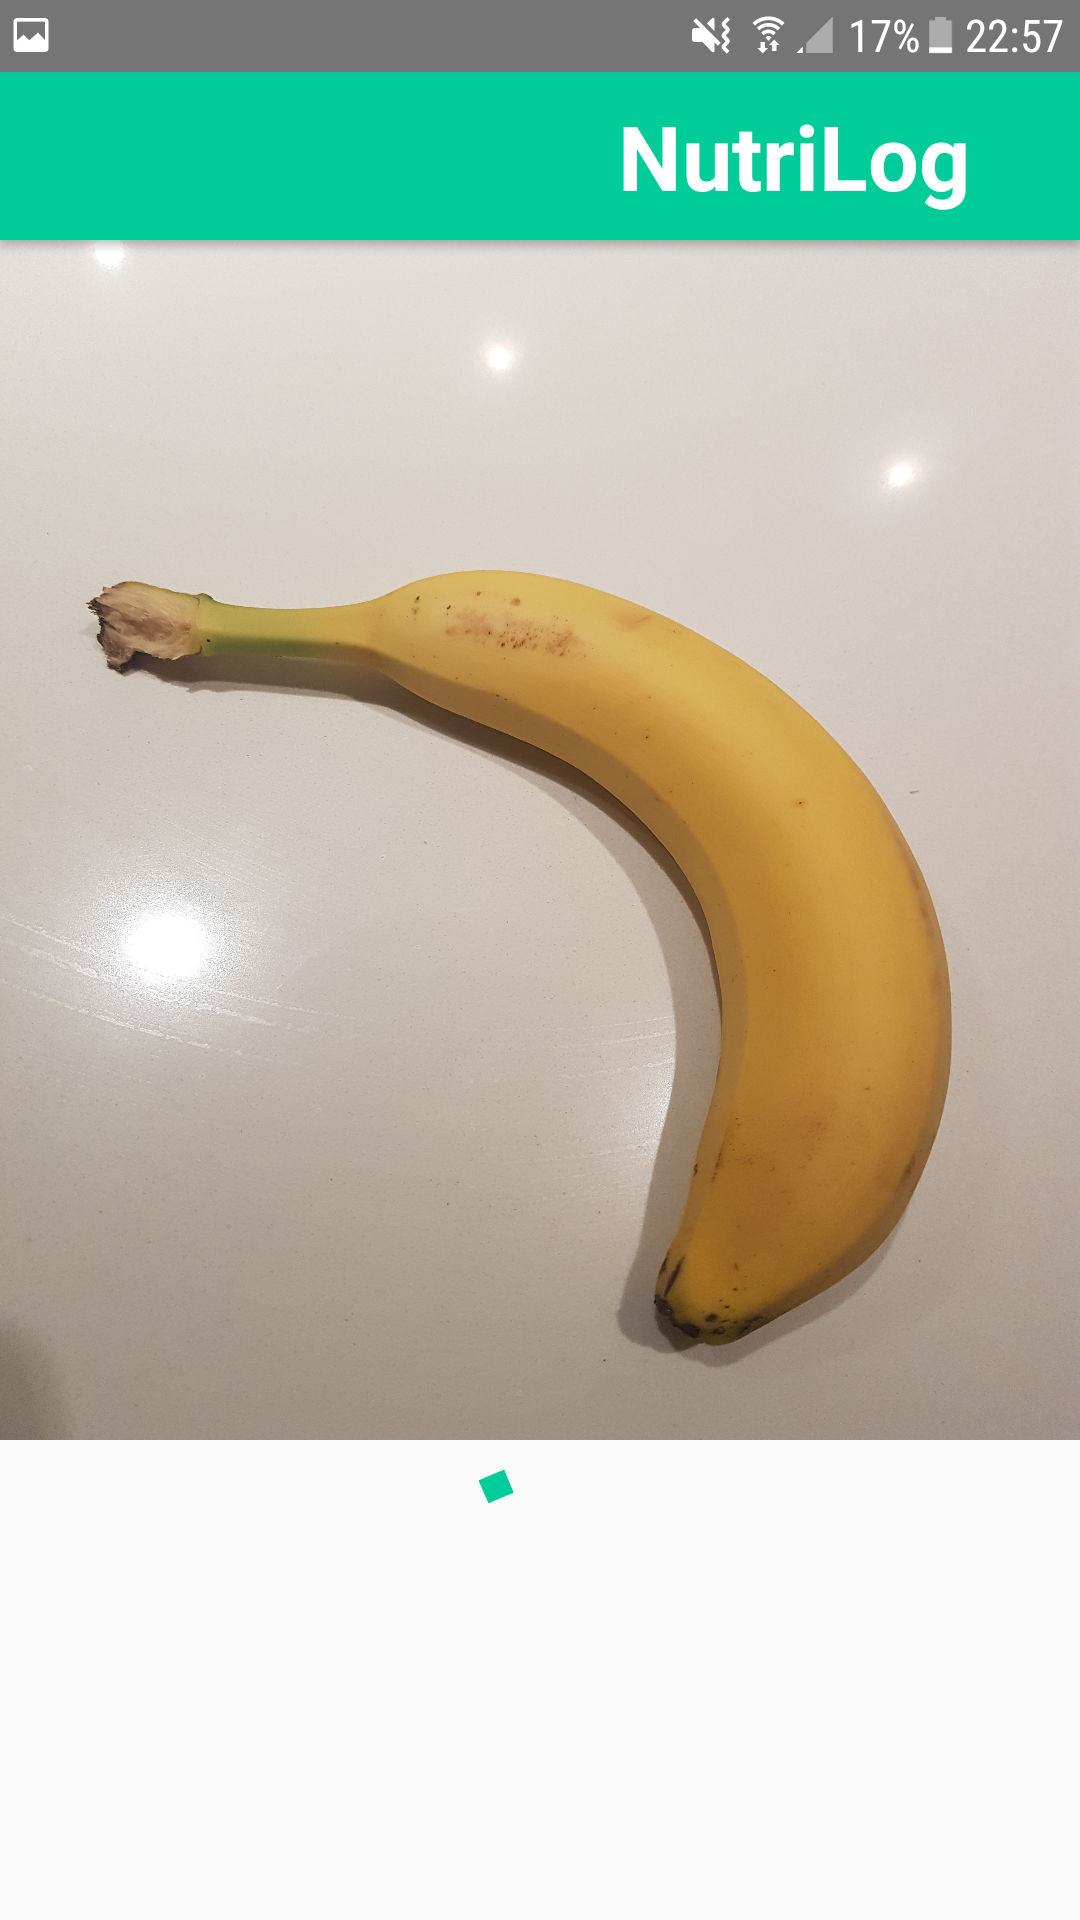
\includegraphics[width=.75\linewidth]{ui4} 
    \caption{Image Processing Activity} 
    \label{fig:ui4}
    \vspace{4ex}
  \end{minipage} 
\end{figure}
\afterpage{\clearpage}

\begin{figure}[h] 
  \label{uiDesign2} 
  \begin{minipage}[b]{0.5\linewidth}
    \centering
    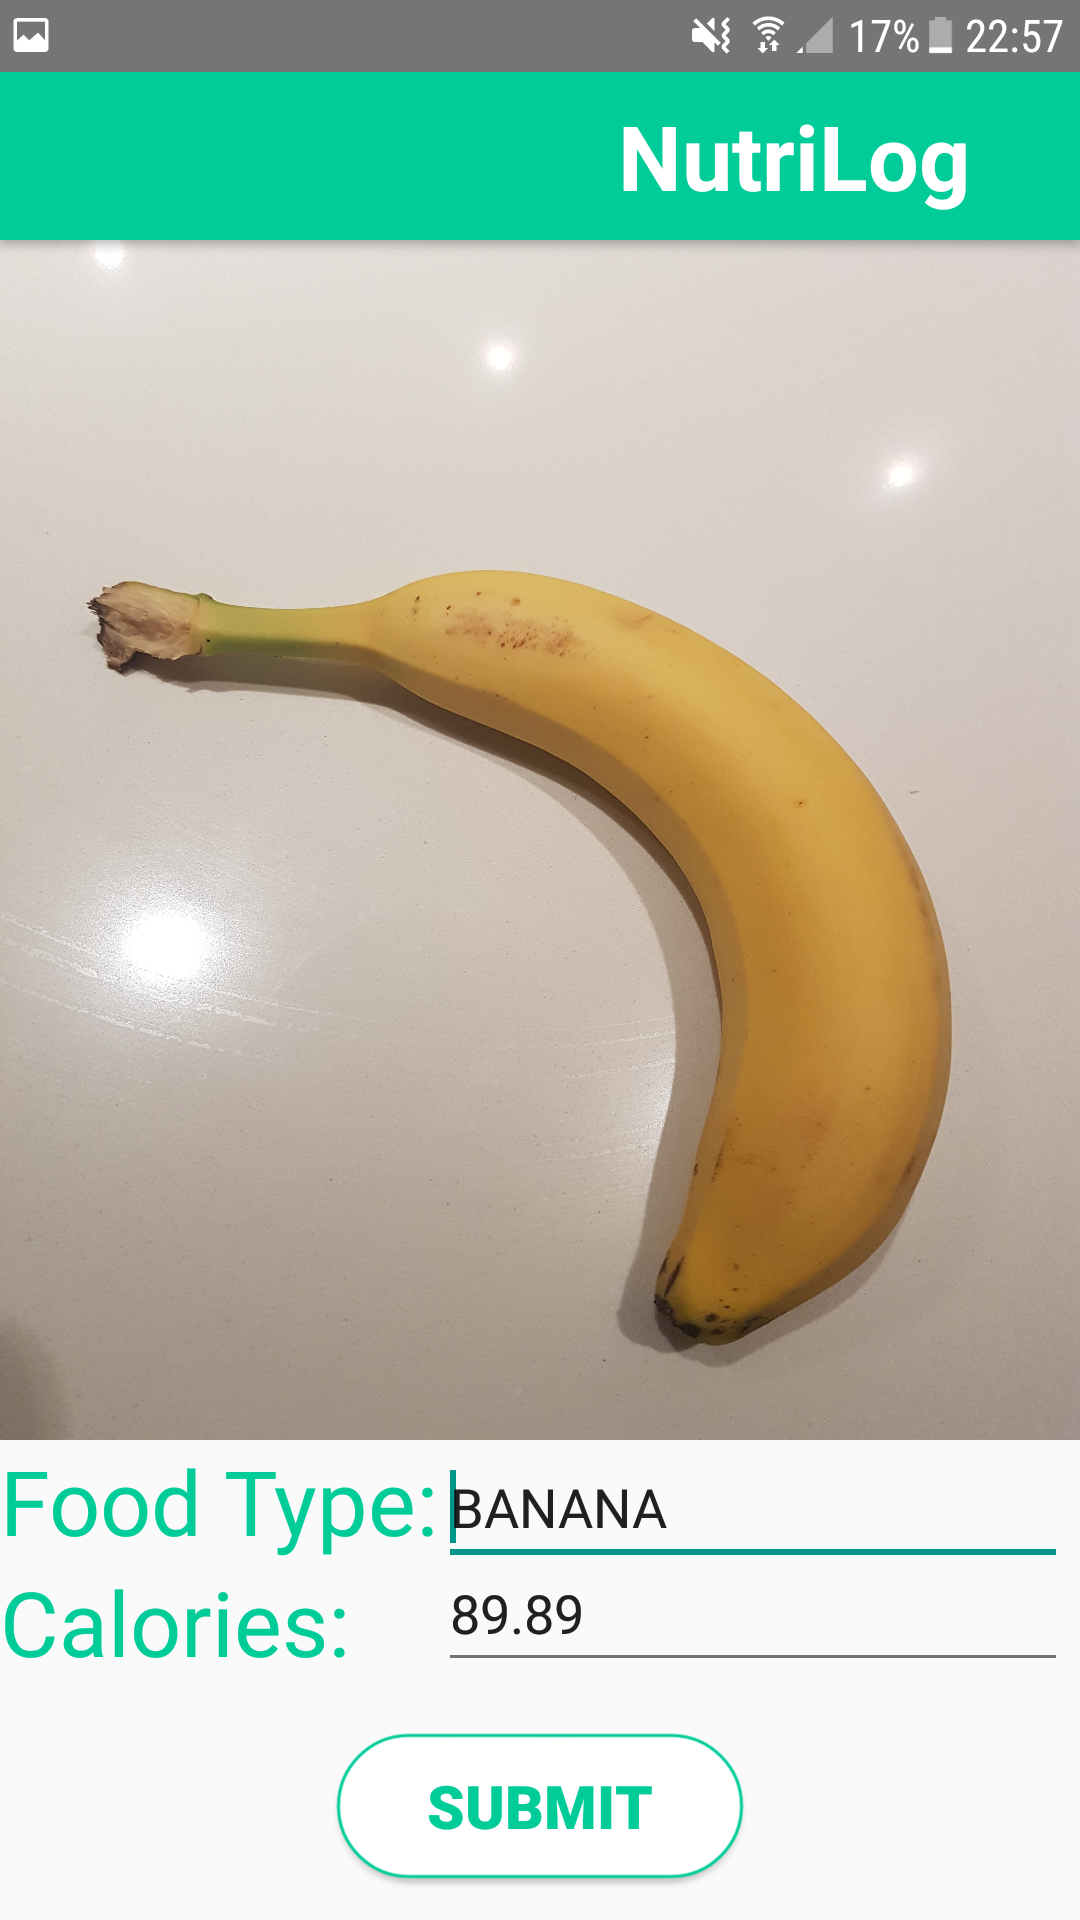
\includegraphics[width=.75\linewidth]{ui5} 
    \caption{Image Submit Activity} 
  \label{fig:ui5}
    \vspace{4ex}
  \end{minipage}%%
  \begin{minipage}[b]{0.5\linewidth}
    \centering
    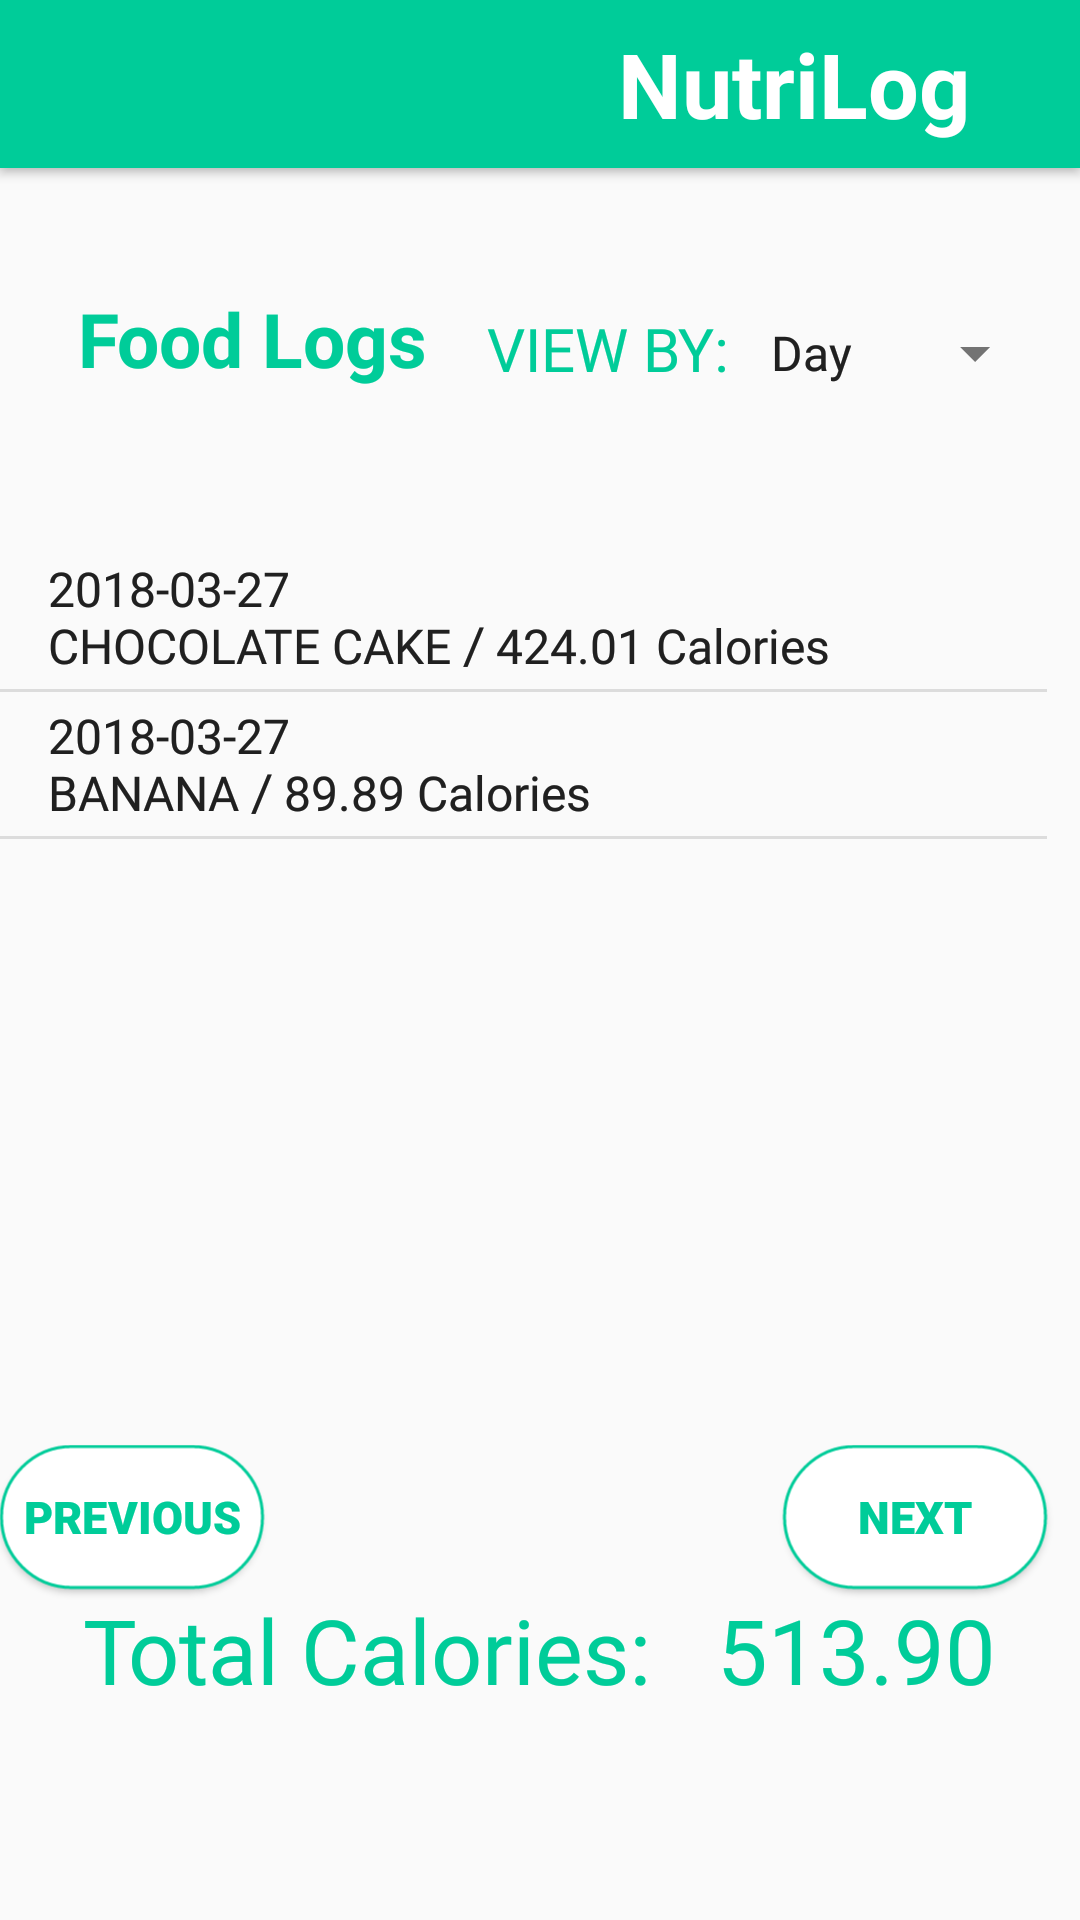
\includegraphics[width=.75\linewidth]{ui6} 
    \caption{FoodLog Day Activity} 
  \label{fig:ui6}
    \vspace{4ex}
  \end{minipage} 
  \begin{minipage}[b]{0.5\linewidth}
    \centering
    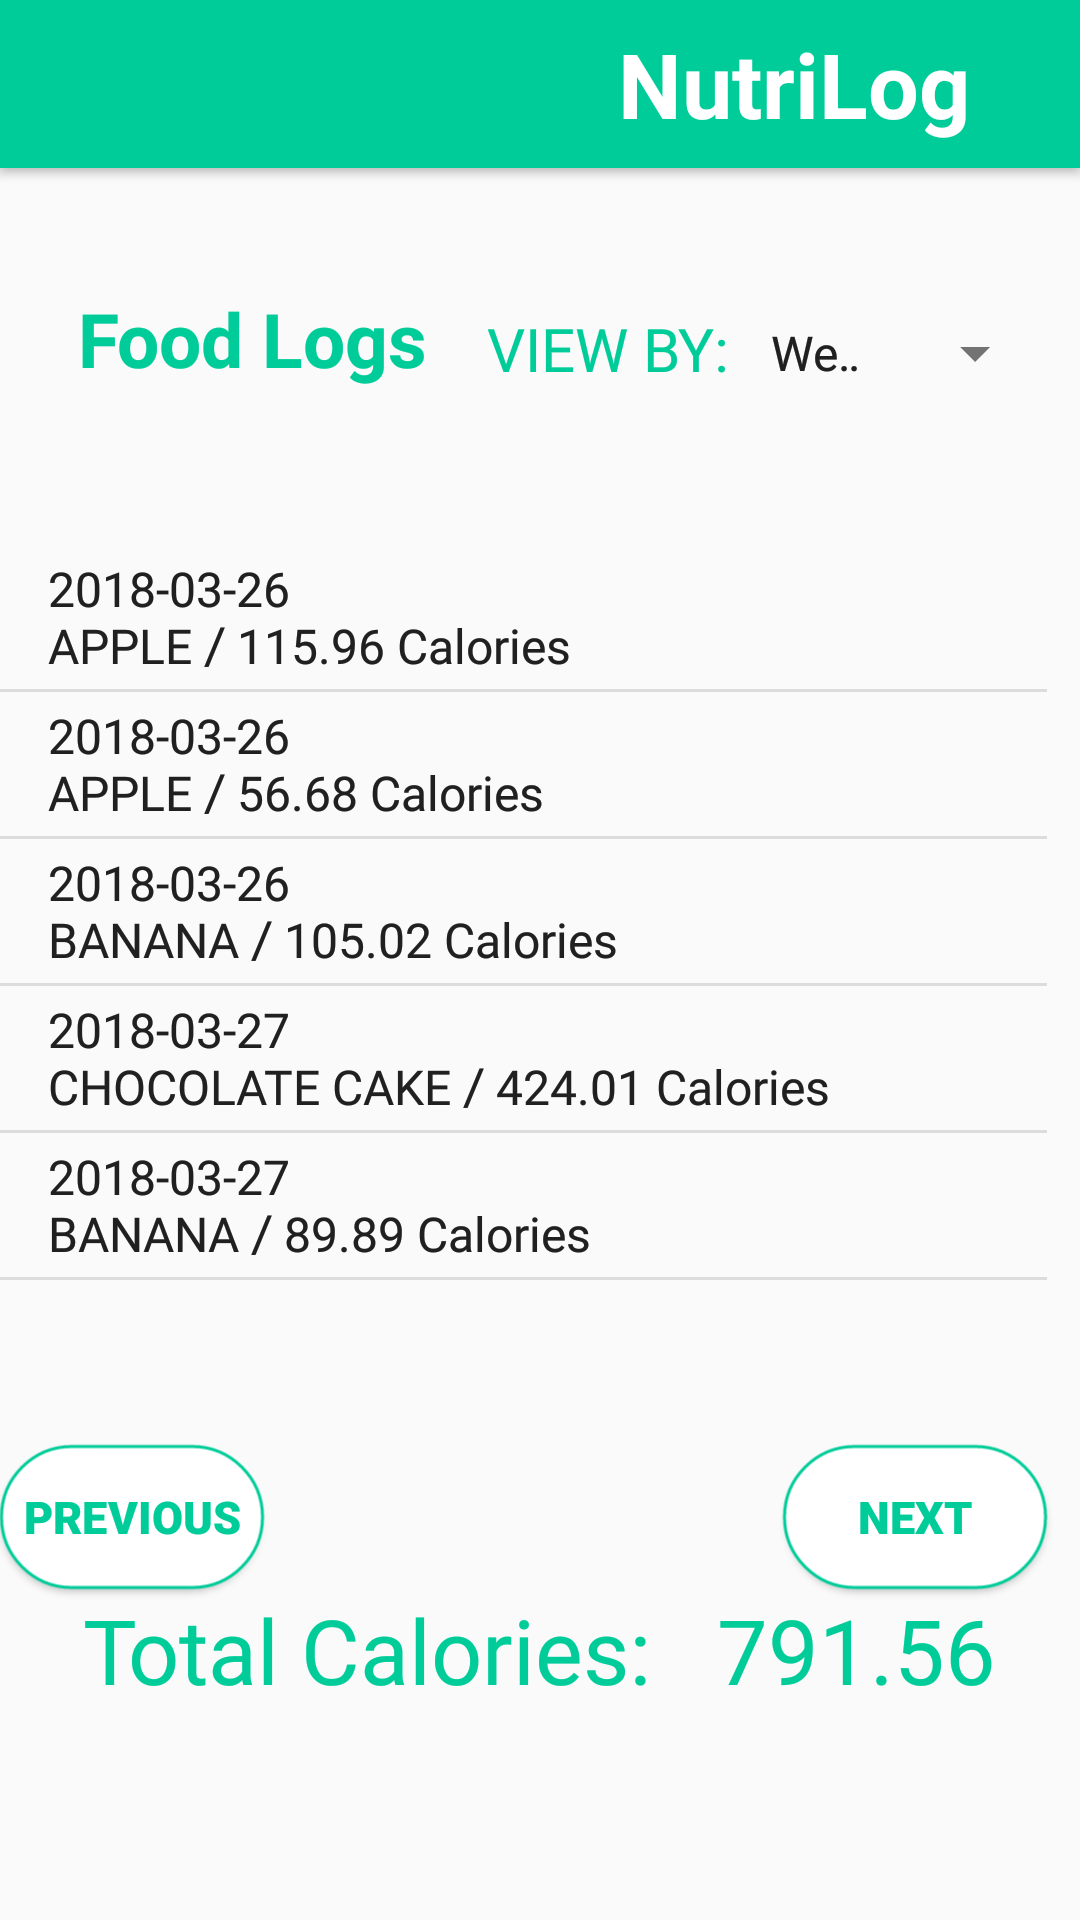
\includegraphics[width=.75\linewidth]{ui7} 
    \caption{FoodLog Week Activity} 
    \label{fig:ui7}
    \vspace{4ex}
  \end{minipage}%% 
  \begin{minipage}[b]{0.5\linewidth}
    \centering
    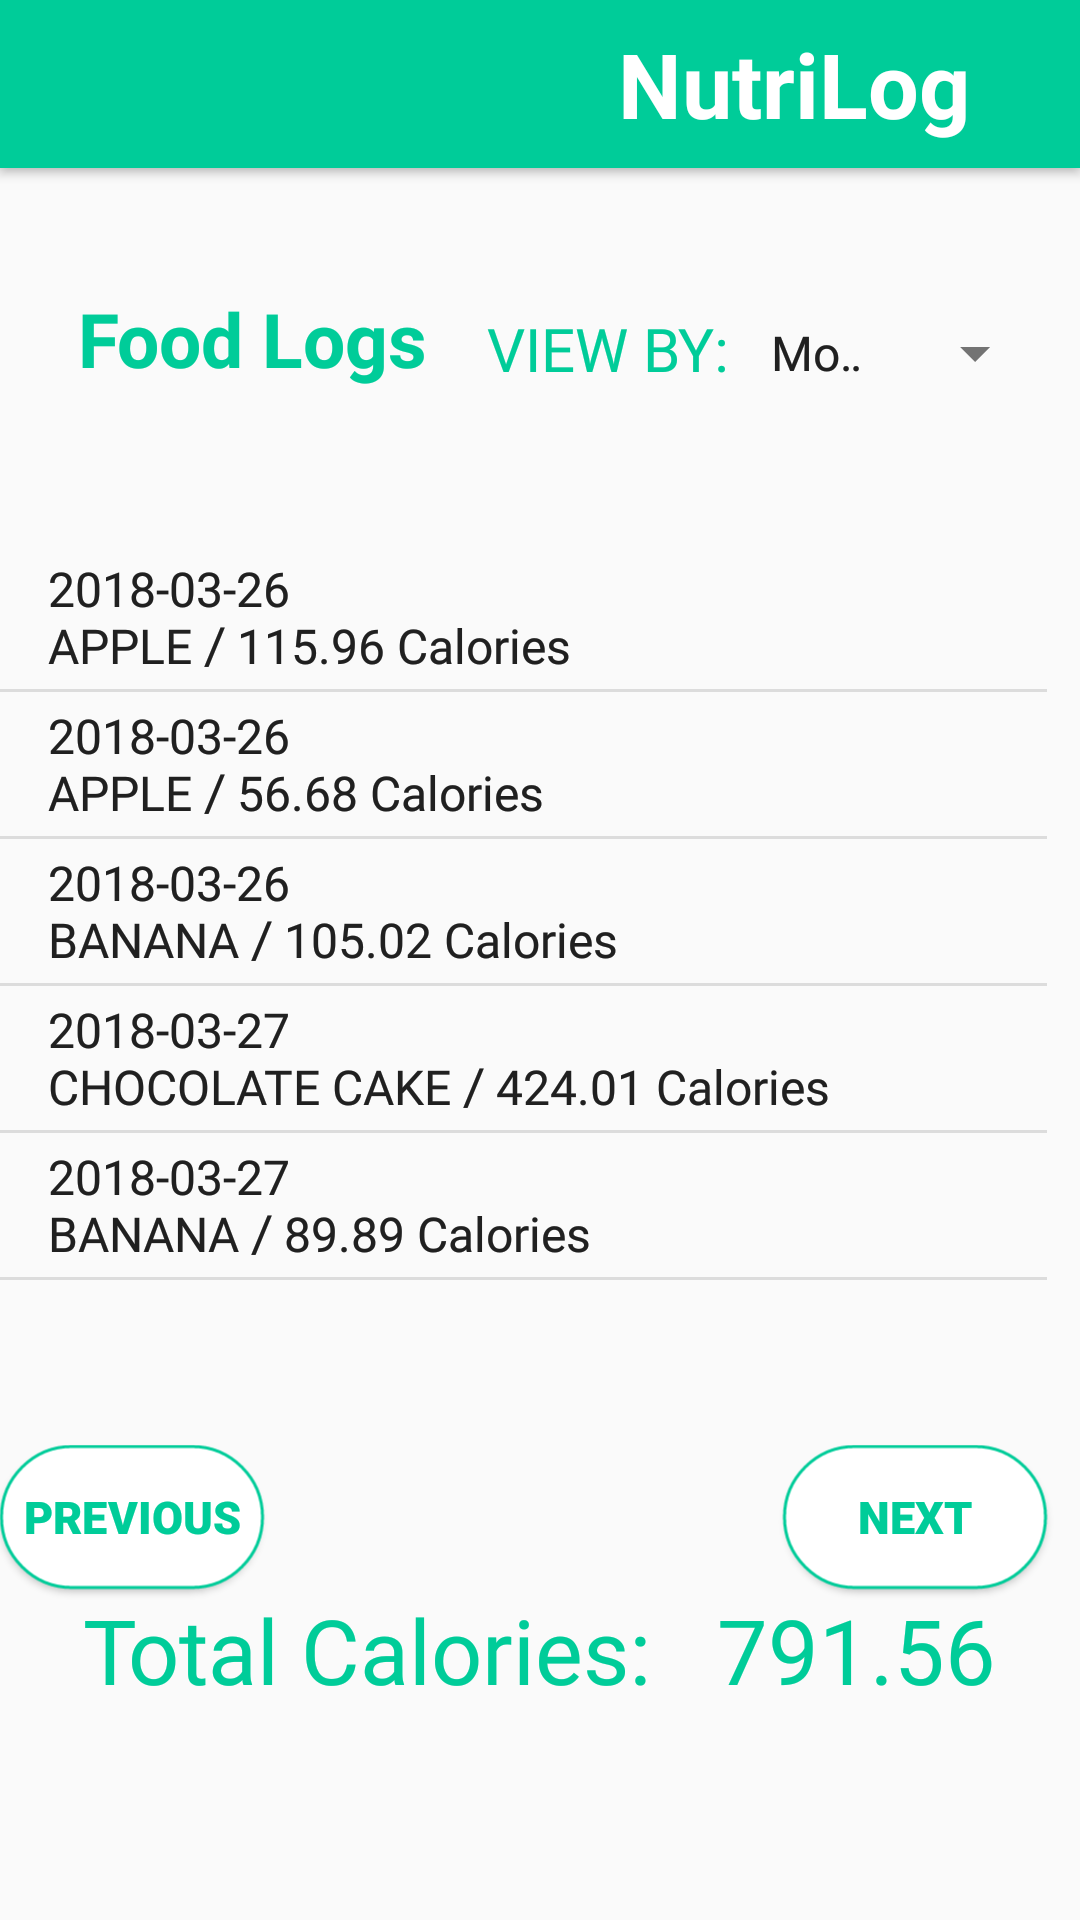
\includegraphics[width=.75\linewidth]{ui8} 
    \caption{FoodLog Month Activity} 
    \label{fig:ui8}
    \vspace{4ex}
  \end{minipage} 
\end{figure}
\afterpage{\clearpage}






